\section{Qu'est-ce qu'un objet audiovisuel numérique ?}\label{sec:dav}
\e{
Dans le monde de l'audiovisuel, certaines notions implicites déterminent la manière dont les professionnels se représentent les objets qu'ils produisent, manipulent, échangent etc. 
L'objectif de cette section est d'expliciter les définitions de ces objets, d'en faire un inventaire (\ref{sec:pv-av}).
Notre démarche ne se limite cependant pas à la vision des professionnels de la production, puisque nous comparons leurs concepts avec ceux d'autres communautés, en vue d'identifier des écarts ou des manques que nous pourrons intégrer dans notre travail.
Ainsi, la communauté des bibliothèques numériques examine plus en détails les relations qui existent entre les résultats d'un processus de création (\ref{sec:pv-bn}). 
La communauté de l'ingénierie documentaire et des sciences de l'information et de la communication invoque quant-à-eux la notion de document, généralement fort absente dans la communauté audiovisuelle, et propose une vision plus fine des différents états de la fabrication et de la consultation d'un contenu audiovisuel (\ref{sec:pv-id}).
Ces deux perspectives apportent une richesse conceptuelle qui, au moment d'examiner les modélisations de l'audiovisuel existantes, nous permettra de mieux identifier ce qu'ils représentent et ne représentent pas.}



\subsection{Du point de vue de l'audiovisuel}\label{sec:pv-av}
Afin de clarifier la notion d'objet audiovisuel, nous présentons la manière dont les professionnels se représentent ses différents composants.
Nous reprenons une liste de définitions proposées par \cite[p.77]{Cox2006} (sauf pour la notion d'\pc{Asset} que nous empruntons à \cite{Austerberry2004}) que nous \ciel{traduisons} et commentons en français : 
\begin{liste}
	\item \pc{Work} (Oeuvre) : \ciel{un travail de création artistique produite ou construite par les efforts conjugués d'une personne ou d'un groupe}.
	Cette définition est clairement reprise du modèle FRBR (voir ci-après) et s'intègre d'ailleurs assez mal avec le reste de la modélisation.

	\item \pc{Essence} : \ciel{toute donnée (numérique) ou signal (analogique) nécessaire à la représentation d'une modalité d'expérience perceptive (visuel, olfactive, auditive etc.)}.

	\item \pc{Material} (Matériel) : \ciel{toute Essence ou combinaison d'Essences (image, son etc.)}. 
	Ainsi, on peut parler de matériel audiovisuel, qui est une combinaison d'Essence audio et visuelle.
	En résumé : Essence/Matériel sont ce que l'on transmet au spectateur, l'Essence se limitant à une modalité.

	\item \pc{Metadata} (Métadonnées) : \ciel{les données qui transportent des informations sur le Matériel -- par exemple des informations d'identification, codage des essences, timeline, propriété intellectuelle etc.}
	Matériel et Essence se différencient des Métadonnées par leur vocation : transmettre une expérience perceptive au spectateur ou transmettre des informations sur le Matériel.

	\item \pc{Content} (Contenu) : \ciel{le Matériel et les métadonnées associées}. 
	Il est particulièrement intéressant de noter l'écart entre cette définition ensembliste et le sens commun. 
	Ici, il s'agit de pouvoir désigner un objet à manipuler, ce qui a de la valeur en terme d'échange, mais non de référer à la signification de l'Oeuvre.
	En résumé : Contenu = Matériel + Métadonnées.

	\item \pc{Instance} : \ciel{une occurrence spécifique et unique de Matériel, Métadonnée ou Contenu}.
	Là encore, l'explicitation de la définition renvoit à un éléments appartenant à trois ensembles. 

	\item \pc{Asset} : \ciel{un asset est ce qui a de la valeur. Le contenu ne suffit pas forcément à représenter un asset. Le propriétaire du contenu doit avoir le droit d'utiliser le matériel avant de pouvoir l'appeler un asset.} 
	En résumé : Asset = Contenu + Droits.
\end{liste}

% On peut résumer ces définitions par l'équation suivante : Asset = Contenu(Matériel + Métadonnées) + Rights.
Cette liste de définition semble intégrer plusieurs manières de se représenter le travail de la production audiovisuelle et ses résultats :
\begin{liste} 

	\item[\g{artistique}] : le travail de création artistique qui aboutit au résultat abstrait d'une Oeuvre. 
	C'est cette réalisation abstraite qui est protégée par la propriété intellectuelle et peut faire l'objet d'une cession de droits.
	Pourtant, la relation entre l'Oeuvre et l'Asset n'est pas établie clairement.

	\item[\g{concrète}] : plusieurs définitions font référence aux résultats concrets de la production (les Instances de Matériel, de Métadonnée et donc de Contenu, les Essences).

	\item[\g{commerciale}] : la notion d'Asset aborde le résultat du travail de production sous l'angle de l'exploitation commerciale. 
	Si on prend l'exemple de la diffusion d'un Contenu qui n'appartient pas à la chaîne, cette diffusion ne peut se faire qu'après achat des droits qui établissent en détails les conditions d'exploitation cédées (zone géographique de diffusion, nombre de rediffusion, limite dans le temps etc.).
	
\end{liste}

% Définition de Media Asset etc. de \cite{Furht2008}.


\subsection{Du point de vue des bibliothèques numériques}\label{sec:pv-bn}
Le \e{Functional Requirements for Bibliographic Records : object-oriented} (FRBRoo) est un modèle conceptuel développé par \cite{Aalberg2008}.
Il vise à faciliter l’échange d’information entre les bibliothèques numériques et les musées. 
Il permet de représenter les personnes participant aux différentes étapes de construction d’un objet culturel, depuis l’idée jusqu’à la réalisation matérielle.

La particularité de cette modélisation est de disséquer les objets culturels dans le but de leur conservation.
Ainsi, le modèle cherche à établir quelles sont les liens généalogiques entre les objets conservés, déterminer les inspirations, les adaptations etc. afin de mettre en évidence des relations culturelles.
Ce souci du détail clarifie les relations entre les objets et par conséquence le processus de création. 
Chaque objet culturel possède trois niveaux de modélisation qui sont présentés dans leur ordre chronologique d'apparition dans le processus de création :
\begin{liste}
	\item le niveau des \e{idées} ou des \e{oeuvres} (\pc{Work}) n’ayant pas pris corps dans une matérialité externe à un sujet (par exemple une mélodie ou une histoire qui nous reste dans la tête). 

	\item le niveau des \e{formes d'expression} (\pc{Expression}) où l'on distingue parmi toutes les formes possibles pour exprimer une idée (une nouvelle écrite, ses traductions, une adaptation de nouvelle en scénario, une lecture de cette nouvelle etc.).
	On se situe à un niveau intermédiaire qui définit des formes abstraites de  réalisation.
	Il faut préciser qu'on parle de forme abstraite dans le sens où il n'existe pas de réalisation concrète, ce qui n'empêche pas de les définir précisement et donc de distinguer de multiples variantes d'expressions :

	\ciel{
	the form of expression is an inherent characteristic of the expression, any change in form (e.g., from alpha-numeric notation to spoken word, a poem created in capitals and rendered in lower case) is a new expression. Similarly, changes in the intellectual conventions or instruments that are employed to express a work (e.g., translation from one language to another) result in the creation of a new expression.} (\cite{Aalberg2008})
	
	\item le niveau des \e{réalisations concrètes} comme les porteurs physiques d’information (\pc{Information Carrier}) portant les expressions (livre, partition, cd-rom etc.). 
	À ce niveau, il faut également distinguer entre l’original (\pc{Manifestation Singleton}) et les copies manufacturées (\pc{Item}) issues d’un modèle de publication (\pc{Manifestation Product Type}). % à rapprocher de la notion de Media Profile dans MPEG-7
\end{liste}

\paragraph{Discussion et comparaison}
Dans la perspective audiovisuelle présentée précédemment, la relation entre Oeuvre et Asset est bien plus floue.
À la fin du processus de création, il apparaît évident que l'on a produit un Asset, mais la notion d'Oeuvre, et donc de l'idée qui a amené à la création, échappe aux systèmes de gestions d'objets audiovisuels.
Ces systèmes ne sont pas fait pour gérer la propriété intellectuelle, ou bien rendre compte des adaptations d'une même idée en plusieurs réalisations.

Par ailleurs, on peut identifier des correspondances entre les notions de FRBR et celles du monde de l'audiovisuel :
\begin{liste}
	\item un \pc{Manifestation Singleton} correspond à la réalisation concrète originale du processus de production, ce qui correspond à la notion de \e{master} dans l'audiovisuel.
	
	\item dans le cadre du numérique, la notion de \pc{Manifestation Product Type} existe dans les cas des documents structurés associés à des feuilles de style.
	On peut noter, que cette notion se rapproche de celle de \pc{MediaProfile} définie dans MPEG-7 à la section \ref{sec:mpeg7}.

	\item un \pc{Item} correspond à une \pc{Instance} de \pc{Contenu} ou de \pc{Matériel}.
	\item un \pc{Information Carrier} correspond à un \e{medium} (media en anglais).

	\item une \pc{Expression} correspond à la notion de \e{format} en audiovisuel.
	Cette notion est centrale puisqu'elle détermine la manière dont la production se déroulera, les moyens attribués, s'il s'agit de l'adapation d'une Oeuvre pré-existante, il faut d'abord vérifier si l'on dispose des droits etc.
	Cette notion est représentée comme une propriété d'un \pc{Contenu} dans ses Métadonnées mais ne permet pas de rendre compte de la relation entre Oeuvre et format d'expression.
\end{liste}





\subsection{Du point de vue de l'ingénierie documentaire}\label{sec:pv-id}
Nous examinons principalement la lignée des travaux de recherche menés initiallement par \cite{Bachimont1998}, formalisés comme une théorie du support numérique dans \cite{bachimont:hdr} puis affinés dans \cite{bachimont:icc}. 
% De nombreux travaux ont repris ce positionnement pour 
Ce positionnement a été approfondi dans le domaine de l'audiovisuel par d'autres auteurs dont \cite{Prie1999}, \cite{Troncy2004}, \cite{Morizet-mahoudeaux2005a}, \cite{Gaillard2008}.

\subsubsection{Les dimensions de l'inscription matérielle}
Ces travaux reposent sur les concepts d'\pc{Inscription}, de \pc{Conte\-nu} et de \pc{Support}. 
La définition d'un \pc{Contenu} permet de relier ces concepts : 
\ciel{
	Un contenu est une forme inscrite sur un support se prêtant à une interprétation à travers laquelle elle fait sens pour quelqu'un ou une communauté.
	C'est donc une \e{forme matérielle interprétable.}} \parcite{bachimont:icc}

Un point à noter est que le contenu est bien une inscription matérielle, non pas le sens que l'on aurait construit de son interprétation.
En tant qu'inscription matérielle, \citeauthor{bachimont:icc} distingue trois dimensions qui caractérisent la manière dont un contenu exprimé sera enregistré, puis restitué.
Dans chacune de ces dimensions (expression, conservation, restitution) intervient une forme, un support et un dispositif, voir la Figure \ref{img:inscriptions}.
Le dispositif a pour objectif de transformer une forme A inscrite sur un support $\alpha$ en une forme B inscrite sur un support $\beta$.

\begin{figure}[ht!]
\centering
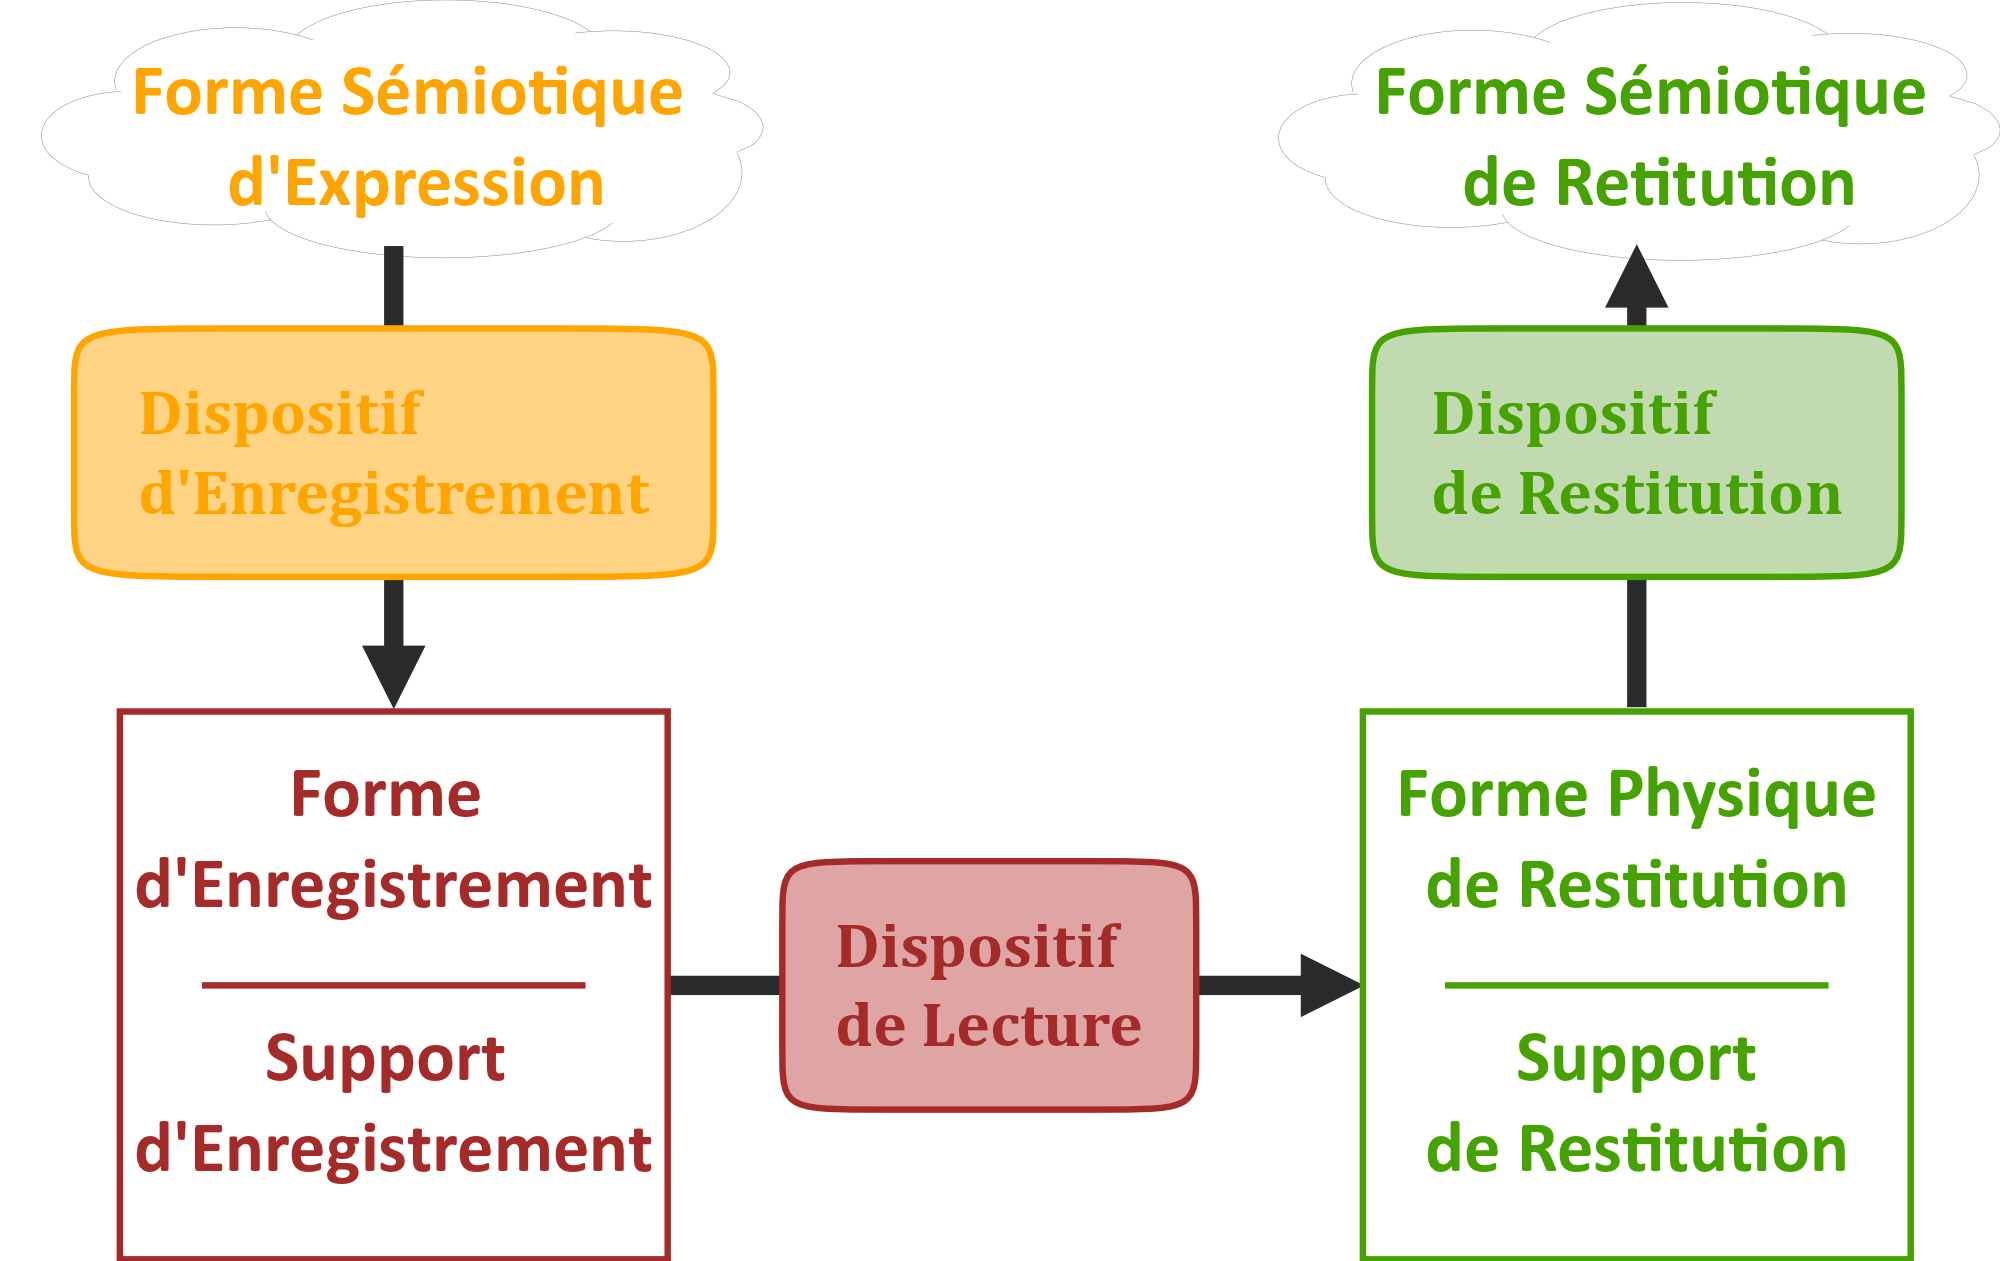
\includegraphics[width=0.7\textwidth]{images/DimensionsInscriptions-v2.png}
\caption{Les dimensions de l'inscription matérielle : forme, support et dispositif}
\label{img:inscriptions}
\end{figure}


\begin{listeni}
	\item \g{dimension de l'expression}
	\begin{liste}
		\item \e{forme sémiotique d'expression} (FSE) : Il ne s'agit pas simplement d'une forme à inscrire, mais bien d'un contenu, puisque l'auteur exprime une intention selon un code sémiotique qui permet à d'autres de l'interpréter.
		La forme sémiotique d'expression est considéré comme volatile et non-permanente, comme la parole ou bien une mélodie sifflée.

		\item \e{dispositif d'enregistrement} (DE) : le dispositif matériel qui réalise l'inscription de la forme d'expression sur un support afin d'assurer sa conservation.
		Cette inscription consiste en une sélection et une configuration de la forme d'expression en une forme d'enregistrement, comme le réalise par exemple un microphone ou bien une caméra.
	\end{liste}

	\item \g{dimension de la conservation}
	\begin{liste}
		\item \e{forme d'enregistrement} (FE) : une forme d'inscription qui assure l'enregistrement, c'est-à-dire la persistance matérielle du contenu sur un support. 
		Par exemple, le code binaire pour un support numérique, un signal mesuré sur une échelle physique quelconque pour l'analogique (magnétique, tension électrique etc.), les lettres de l'alphabet pour l'écriture etc.

		\item \e{support d'enregistrement} (SE) : l'objet matériel sur lequel on inscrit une forme pour conserver et préserver le contenu.
		Par exemple, le papier pour un texte, un 45 tours pour la musique, une mémoire magnétique (disque dur etc.) ou optique (CD etc.) pour le numérique, une cassette vidéo pour une vidéo analogique etc.

		\item \e{dispositif de lecture} (DL) : le dispositif matériel qui réalise la transformation de la forme d'enregistrement en une forme physique de restitution.
		Par exemple, un tourne-disque pour les 45 tours, un ordinateur avec un lecteur multimédia pour une vidéo numérique, un magnétoscope pour une cassette vidéo etc.
	\end{liste}

	\item \g{dimension de la restitution}
	\begin{liste}
		\item \e{forme physique de restitution} (FPR) : une forme sous laquelle l'inscription est présentée pour être perceptible.
		Par exemple, des pixels de couleurs pour une vidéo, une onde sonore pour une musique etc.
		Les normes MPEG-1 et MPEG-2 définissent des techniques d'encodageet de compression d'images et de vidéos.
		Il s'agit donc de normes qui permettent la numérisation de la FPR.
		
		\item \e{support de restitution} (SR) : il s'agit de l'objet matériel sur lequel la restitution du contenu s'inscrit, ce qui permet à un lecteur d'appréhender un contenu par ses sens. 
		Par exemple, un écran pour un signal visuel ou bien l'air ambiant pour le son.
		Cet élément est relié au dispositif de lecture, qui se contente de fournir une forme sans la rendre perceptible à son lecteur, ainsi qu'au dispositif de restitution, qui lui permet au lecteur de l'interpréter.
		
		\item \e{dispositif de restitution} (DR) : le dispositif matériel qui permet de transformer une forme physique en une forme sémiotique.
		Il peut s'agir d'un téléviseur ou d'un écran d'ordinateur pour une forme visuelle, de haut-parleurs pour une forme sonore.
		
		\item \e{forme sémiotique de restitution} (FSR) : une forme de représentation intelligible par l'utilisateur qui en connaît les codes sémiotiques.
		Les formes sémiotiques usuelles sont l'image, la musique, le bruit, la parole etc.
	\end{liste}
\end{listeni}

L'intérêt de cette définition du contenu par état (forme/support) est également de pouvoir introduire la notion de document et de formes documentaires, complètement absente des deux premières perspectives que nous avons examinées.


\subsubsection{Le document numérique}\label{sec:docnum}
\cite{Morizet-mahoudeaux2005a} définissent un document comme un contenu qui peut servir de référence par sa consistance matérielle dans le temps : \ciel{a document is a \e{content} instituted by a \e{publication act}, written down a medium, which possesses a \e{spatial} and \e{temporal delimitation}}.

\begin{liste}
	\item \e{permanence dans le temps} : \ciel{la consistance des signes matériels qu’il porte doit être assurée quelque soit le moment de leur consultation.} \parcite{Bottini2010}

	\item \e{délimitation spatiale} : un document se définit par ce qu'il contient et ce qu'il ne contient pas.
	C'est par ses frontières que le document ouvre la possibilité de sa lecture et de son interprétation.

	\item \e{délimitation temporelle} : la naissance d'un document est institué par un acte de publication, c'est-à-dire le moment où l'on arrête de faire varier sa forme matérielle, pour le faire rentrer dans une sphère médiatique.

	\item \e{intentionnalité} : le document est porteur d'une signification qui ne se résume pas à sa forme matérielle.
	On peut distinguer les documents possédant une intentionnalité \e{a priori} (l'objet matériel a été créé pour porter une intentionnalité documentaire) et ceux dont on attribue une intentionnalité \e{a posteriori} (par exemple, des outils de chasse retrouvés par un archéologue qui les interprètent pour reconstruire les habitudes de l'époque).
\end{liste}


Pour \cite{Leleu-Merviel2004}, le document comporte à la fois une dimension \e{sémiotique} qui renvoit au contenu (signes et sens), \e{technique} qui renvoit aux données (format d'enregistrement, codage et transmission de signaux) et \e{médiatique} qui renvoit à des processus de socialisation, de diffusion, de réception et de consultation.
\cite{Leleu-Merviel2005} décrit cette dernière dimension comme étant la dimension d'accès aux données, un accès qui peut être organisé spatialement et temporellement :
\begin{liste}
	\item la \e{scénique} est la manière de transposer des données en une réalité concrète : \ciel{la forme visuelle et sonore de l’inscription spatiale des fragments}. %FPR+SR
	\item la \e{scénation} est la manière de restituer temporellement à l'utilisateur les fragments d'un document : \ciel{la structure organisée d’événements et/ou d’états avec lesquels l’utilisateur est effectivement mis en interaction}. %DR+FSR
\end{liste}

On retrouve dans cette définition, la caractérisation de l'inscription matérielle faite par \cite{bachimont:icc} avec les correspondances suivantes : 
\begin{liste}
	\item les données correspondent à la FE, l'enregistrement en binaire, inaccessible et illisible pour l'humain. 
	\item la dimension sémiotique renvoit à la FSR ainsi qu'à ses structuration.
	\item la scénique renvoit à l'association FPR + SR qui rend perceptible le contenu.
	\item la scénation renvoit à l'association FSR + DR qui conditionne l'interprétation du contenu.
\end{liste}

Cette définition développe celle proposée antérieurement par le réseau thématique pluridisciplinaire 33 (RTP-DOC, \cite{Pedauque2003}) qui fait référence dans les communautés scientifiques engagées dans les questions documentaires.
Leur définition du document comporte trois dimensions similaires : le document comme \e{forme} (la dimension matérielle dans laquelle s’incarne le contenu et qui permet sa manipulation), le document comme \e{signe} (il est porteur d’un sens intentionnel), et le document comme \e{médium} (sa dimension sociale, d'échange et de communication).

 


\subsubsection{Unité de contenu et structures documentaires}\label{sec:uc-sd}
La distinction entre \e{forme physique de restitution} (FPR) et \e{forme sémiotique de restitution} (FSR) sera essentielle pour l'examen des modélisations de l'audiovisuel.
Un changement de la FSR impacte la signification du contenu, alors que les changements sur la FPR ont une conséquence sur le plan perceptif, mais pas forcément sur la signification (un pixel mort ne change pas le sens d'une image).
Comme nous le verrons plus tard (\ref{sec:codesc}), beaucoup de modèles se focalisent sur la FPR, c'est-à-dire sur la caractérisation du signal par des descripteurs de bas-niveau que l'on pourrait qualifier d'objectif (texture, couleur, forme etc.).

La modélisation de la FSR se fonde sur une interprétation de la forme matérielle du contenu pour dégager ce que \cite{Prie2000} appelle des \e{structures documentaires}.
Une structure documentaire découpe le contenu en unités suivant une grammaire de (dé)composition.
\citeauthor{Prie2000} considère ainsi que \ciel{toute structure est sémantique et fait partie d'une structure d’indexation conceptuelle} qui renvoit donc à une utilisation \ciel{dans le cadre d'une tâche qui peut être une tâche de présentation}.
L'indexation conceptuelle est définie commme \ciel{explicitation de structures et de concepts contenus dans les documents numériques ou qui leur sont associés, pour mieux les exploiter}.
On construira donc des structures différentes suivant l'exploitation du contenu visée, qu'il s'agisse de produire une interprétation pour faciliter l'accès au contenu, de manipuler le contenu ou bien d'en fournir une présentation. 

\citeauthor{Prie2000} distingue ainsi le cas particulier de l'écriture.
Il s'agit d'une tâche à part où \ciel{l’intentionnalité de l’auteur se retrouve plus ou moins dans les structures documentaires} qu'il définit. 
Ces structures expriment des \ciel{connaissances \e{auctoriales} premières}, dans le sens où elles constituent le document et permettent sa médiatisation auprès d'un lectorat.
Cette structure documentaire première renvoit également à un genre documentaire, où elle puise une \ciel{une structure de présentation \e{canonique}}, souvent appelée structure logique par d'autres auteurs.
La notion de genre, amène à la notion de tradition de lecture, dont les éléments de structure canoniques prescrivent une interprétation du document.
Les auteurs peuvent ainsi identifier des communautés de lecteurs par les genres documentaires qu'elles mobilisent dans leurs activités.

La structure première ou canonique définit par l'auteur sert ensuite à d'autres communautés pour établir leur propre structure documentaires en fonction de leurs usages.
Lorsque plusieurs structures sont associées à un document, \cite{Abascal2003} et \cite{Abascal2004} parlent alors de documents \ciel{multistructurés}, chacune répondant aux contraintes d'un usage.

La multiplicité des structures documentaires n'éclaire pas pour autant sur leur nature.
\cite[p.191-192]{bachimont:icc} propose ainsi de distinguer entre quatre niveaux :
\begin{liste}
 	\item \e{niveau physique} : le document est avant tout un assemblage de formes matérielles (unités de contenu), organisées et destinées à faire sens pour un lecteur.

 	\item \e{niveau de typage du contenu} : chaque unité de contenu possède un type qui détermine sa sémantique et les manipulations qu'il peut subir.
 
 	\item \e{niveau syntaxique} : des règles syntaxiques (grammaire) tirent parti du typage des unités de contenu pour régir leur organisation au niveau physique. 

 	\item \e{niveau conceptuel} : le typage d'une unité de contenu lui associe également une signification conceptuelle, indépendante des règles syntaxiques (comme \citeauthor{Prie2000} le fait remarquer avec les structures documentaires).
\end{liste}


La caractérisation de ces différents niveaux nous renvoit aux besoins de modélisations exprimés en \ref{sec:bm-av} (\g{B1 : autonomie} et \g{B2 : réutilisabilité}).

% on propose une modélisation logique du document qui repose sur la vision des contributeurs à sa production.


% paragraph{Discussion et comparaison}

% \paragraph{La personnalisation document}
% \ciel{
% Cependant en numérique, les fragments existaient, au moins potentiellement, dans la mémoire de la machine, ce n’est que leur actualisation sur l’écran et la forme qu’elle prend qui se construit dans l’ici et maintenant de l’interaction. 
% Celle-ci est donc nécessairement volatile. De plus, elle change à chaque fois.
% Ainsi c’est l’affichage, [\dots] qui varie, mais non le document lui-même tel qu’il est mémorisé au niveau des données.}

% \ciel{
% conserver, retrouver l’information n’est pas suffisant. 
% Pour qu’elle puisse être utile, il faut qu’elle puisse être exploitée, c’est-à-dire traitée et rapprochée d’autres de façon à produire de l’information nouvelle. 
% Produire du sens n’est, pour l’essentiel, que rapprocher des informations disparates jamais rassemblées auparavant.} (\cite{Balpe1990})

% % Deux pistes proposées par SLM : 
% Il est alors possible de construire des assemblage cohérent de fragments le temps d'une consultation (d'un affichage) par un utilisateur (documents virtuels personnalisables).
% Plus on a de connaissance sur son activité, ses tâches, ses compétences propres, plus il est alors possible de rendre cette assemblage pertinent. 

% Il est aussi possible de mettre à profit la description des documents pour construire des notions de voisinage indépendamment du profilage des utilisateurs. 
% La proximité entre deux documents pourra s'évaluer d'autant de manière qu'il y a de critères descriptifs.
% Ainsi, des informations auparavant éparpillées dans des documents papier différents pourraient être regroupés. 

